\section{Background}
\label{sec:background}
UP-SSO is compatible with OIDC, and achieves privacy protections based on Intel SGX.
%Here, we provide a brief introduction on OIDC and the SGX.
\subsection{OpenID Connect and PPID}
OIDC~\cite{OpenIDConnect} is an extension of OAuth 2.0 to support user authentication,
 and one of the most prominent SSO protocols.
%Same as other SSO protocols~\cite{SAMLIdentifier}, OIDC involves three entities, i.e., {\em users}, the {\em identity provider (IdP)}, and {\em relying parties (RPs)}.
%PPID is suggested in OpenID Connect protocol to protect the user from a possible correlation among RPs.

\begin{figure}[t]
  \centering
  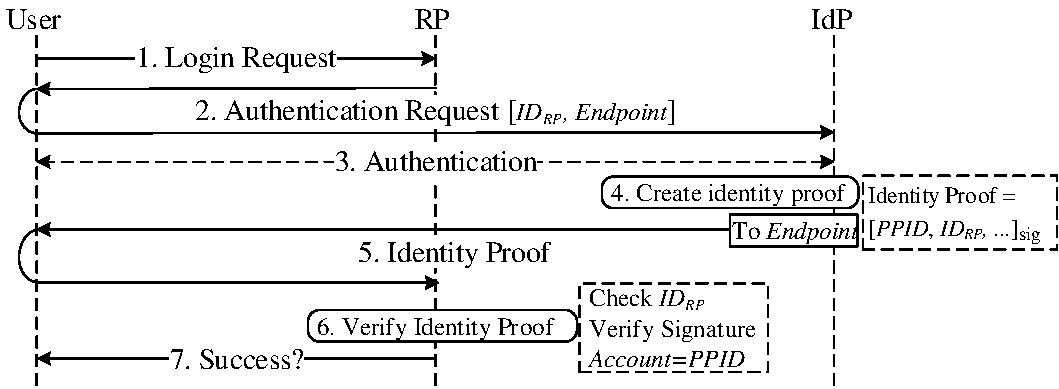
\includegraphics[width=\linewidth]{fig/OIDC1.pdf}
  \vspace{-4mm}
  \caption{The implicit protocol flow of OIDC.}
  \label{fig:OpenID}
  \vspace{-4mm}
\end{figure}

\vspace{1mm}\noindent\textbf{Implicit Flow of User Login.}
The implicit flow is the typical user login flow of OIDC.
% ����ģʽ�Ͳ�д�ˣ��ڱ����У�д��û������
%OIDC supports three processes for the SSO authentication session, known as {\em implicit flow}, {\em authorization code flow} and {\em hybrid flow} (i.e., a mix-up of the previous two). Here, we choose the OIDC implicit flow as the example to illustrate the protocol.
%In the implicit flow, an {\em id token} is generated as the identity proof, which contains a user identifier, an RP identifier, IdP's identifier, the validity period, and other requested attributes.
%The IdP signs the id token using its private key to ensure integrity.
As shown in Figure~\ref{fig:OpenID},
at the beginning, a user attempts to log into an RP (Step 1).
The RP constructs a request for identity proofs,
 which is redirected by the user to the IdP.
This request contains $ID_{RP}$ and other optional attributes (Step 2).
If the user is not authenticated, the IdP initiates an authentication process (Step 3).
Then, the IdP signs $ID_{RP}$ and the user's unique identity (or PPID) into an identity proof, and sends it back to the RP (Steps 4 and 5).
The RP finally verifies this identity proof, extracts the user identity, and returns the result (Steps 6 and 7).
\begin{comment}
\item[1] At the beginning, user attempts to log in to an RP.
\item[2] RP constructs a request for identity proof, which is redirected by the user to the corresponding IdP. The request contains $ID_{RP}$, RP's endpoint other attributes.
\item[3] If the user has not been authenticated yet, the IdP performs an authentication process.
\item[4] IdP signs the $ID_{RP}$ and PPID as the identity proof.%If the RP's endpoint in the request matches the one registered at the IdP, it generates an identity token. Otherwise, IdP generates a warning to notify the user about potential identity proof leakage.
\item[5] IdP sends the identity proof back to the RP.
\item[6] The RP verifies the id token, and extracts user identifier.
\item[7] Finally, RP returns the authentication result to the user.
\end{comment}

\vspace{1mm}\noindent\textbf{Pairwise Pseudonymous Identifier (PPID).}
%PPID is the user identifier provided by IdP identifying a user.
Different from the unique user identity at the IdP,
 a PPID is an RP-specific user identity.
That is, while a user visits different RPs, the IdP will provide a different but constant user identity for each RP.
NIST~\cite{NIST2017draft} suggests that PPIDs should be generated randomly and assigned by the IdP,
 or derived from a user's information if the derivation is irreversible and unguessable.
%that PPID should be used to prevent the user's account at the IdP from being easily linked at multiple RPs through use of a common identifier.
%It also suggests that PPID should be either generated randomly and assigned to users by the IdP, or derived from other user's information if the derivation is done in an irreversible, unguessable manner (e.g., using a keyed hash function with a secret key).
%For example, we have learned that, MITREid Connect, a popular open-source OIDC project, generates PPID using a secure random number generator, and stores the key-value map of corresponding RP and PPID.


\subsection{Intel SGX}
Intel Software Guard Extensions (SGX)~\cite{costan2016intel}
 is the hardware-based security  mechanism provided by Intel processors.
A task protected by SGX runs within an enclave,
    and this enclave is able to attested its run-time integrity to remote entities.
%It offers memory encryption that isolates specific application code and data in memory.
%It allows user-level code to allocate private regions of memory, called enclaves~\cite{costan2016intel}, which guarantees the running codes are well protected from the adversary outside the enclave.

\vspace{1mm}\noindent\textbf{Enclave.}
The enclave’s code and data is stored in Processor Reserved Memory (PRM).
PRM cannot be directly accessed by other software, including system software and System Management Module code (Ring 2).
The Direct Memory Access (DMA) of PRM is also unavailable, as enclave is protected from other peripherals. That is, while the application is running inside the enclave, even the device owner cannot break its security, such as accessing or tempering the application's data.



\vspace{1mm}\noindent\textbf{Remote Attestation.}
Remote attestation enables the software inside an  enclave to attest to a remote entity that it is trusted.
%That is, during the attestation, the remote entity would receive an SGX attestation signature, containing the enclave’s measurement (a measurement of the code and data loaded in enclave).
The SGX remote attestation allows a player to verify the application's identity, intactness (never tampered), and that it is running securely within an enclave.
Moreover, with the remote attestation, the secure key exchange between the player and remote enclave application is also available.% even the application runs in a malicious environment.


\subsection{Existing Privacy-Preserving Solutions for SSO}
\label{sec:existingSolution}
NIST~\cite{NIST2017draft} suggests that the SSO should prevent user's trace from being tracked by both RP and IdP.
%The pairwise user identifier (e.g., PPID) is used in some SSO protocols, such as SAML~\cite{SAML} and OIDC~\cite{OpenIDConnect}.
Some protocols simply hide the RP's identity from IdP, such as SPRESSO~\cite{SPRESSO} (using encrypted RP identifier) and BrowserID~\cite{BrowserID} (RP identifier is added by user). 
An encrypted RP identity is bound in identity proofs by the SPRESSO IdP,
    while the BrowserID IdP firstly binds the user identity and a key pair and the user will bind the RP identity by itself using the certified key pair.
    However,  they are not defensive to RP-based identity linkage, and
PPID cannot be integrated in this type of solutions,
     as the IdP cannot assign the PPID based on an \emph{unknown} RP identity.
%However,  they are not defensive to RP-based identity linkage, and cannot integrate PPID.
%Moreover, an analysis on Persona found IdP-based login tracing could still succeed~\cite{FettKS14, BrowserID}.

There is also another method that prevents both IdP and RP from knowing user's trace based on zero-knowledge algorithm, such as EL PASSO~\cite{ZhangKSZR21} and UnlimitID~\cite{IsaakidisHD16}. 
In such systems, the user needs to keep a secret $s$ and requires IdP to generate an identity proof for blinded $s$. Then user has to prove that she is the owner of $s$ without exposing $s$ to RP.
It can protect user from both IdP-based login tracing and RP-based identity linkage.
However, whenever a user tries to visit RP at a new device, she must import  $s$ into this device. Thus, it is not convenient for user's login on multiple devices.
%However, this type of solution requires user should remember a secret representing his identity, which is not convenient for login on multiple devices.

\subsection{Extended Related Works}
\noindent\textbf{Security analysis of SSO systems.} Various attackers were found accessing the honest user's account at RP by multiple methods.
Some attackers exploit the vulnerabilities of user's platforms to steal  identity proof (or cookie)~\cite{WangCW12,ArmandoCCCPS13}.
Some other attackers temper the identity proof to impersonate an honest user, such as XSW~\cite{SomorovskyMSKJ12}, RP's incomplete verification~\cite{WangCW12,WangZLG16,MainkaMSW17}, and IdP spoofing~\cite{MainkaMS16,MainkaMSW17}.
Some IdP services did not bind the identity proof with a corresponding RP (or the honest RP did not verify the binding), so that malicious RP can leverage the received identity proof to access to another RP~\cite{WangZLG16,MainkaMS16,MainkaMSW17}.
The formal analysis is also used to guarantee the security of SSO protocols~\cite{FettKS16,FettKS17}.

\vspace{1mm}\noindent\textbf{Authentication systems built based on Intel SGX.} Intel SGX has been used in enhancing the security and privacy of authentication systems. Rafael et al.~\cite{CondeMW18} offer the credential protection approach based on SGX, which prevents an adversary from stealing a user's credential at server side. P2A~\cite{SongWLOWL20} is proposed to protect user's privacy. It enables a user to generate an identity proof locally while the registration, update, freeze/thaw, and deletion of identities are managed in a blockchain. Therefore, a user can visit a service without exposing his real identity.



\begin{comment}
\item {\noindent\textbf{Hiding RP Identities from the IdP.}} SPRESSO~\cite{SPRESSO} and BrowserID~\cite{BrowserID} were proposed to protect user privacy against the IdP by hiding RP identities.
An encrypted RP identity is bound in identity proofs by the SPRESSO IdP,
    while the BrowserID IdP firstly binds the user identity and a key pair and the user will bind the RP identity by itself using the certified key pair.
PPID cannot be integrated in this type of solutions,
     as the IdP cannot assign the PPID based on an \emph{unknown} RP identity.
\item {\noindent\textbf{Proving user identity based on zero-knowledge proof. }}In this type of solution, such as EL PASSO~\cite{ZhangKSZR21}, the user needs to keep a secret $s$ and requires IdP to generate an identity proof for blinded $s$. Then user has to prove that she is the owner of $s$ without exposing $s$ to RP.
It can protect user from both IdP-based login tracing and RP-based identity linkage.
However, whenever a user tries to visit RP at a new device, she must import  $s$ into this device. Thus, it is not convenient for user's login on multiple devices.
\end{comment}